% Example command: latexmk -pdf -shell-escape mytemplate.tex

\documentclass{mytemplate}
%\documentclass[10pt]{article}

\usepackage{minted}

% set minted fontsize
\setminted{fontsize=\small,baselinestretch=1}

\title{System Dynamics and Control} % The title.
\project{Spacecraft Dynamics and Control}
\author{Homework 2\\ % topic
Chih-An Lai\\ % Your Name
Technische Universität Berlin % Organization.
}
%\date{} % It can specify a certain day.

\begin{document}

\maketitle

\tableofcontents

\section{How to insert the code}
\inputminted[fontsize=\footnotesize,frame=single,label=least\_cost\_function.m]{octave}{least_cost_function.m}

 \section{How to type complicate equation.}
A demonstration of aligned equation.
\eq{&x^1+x^2\\ % & for alignment
&+x^2\\}

A equation without reference number.
\eq{f(x)  = \int \left( \frac{x^2 + x^3}{1} \right)dx}

A equation with reference number.
\eqr{f(x) = \int \left( \frac{x^2 + x^3}{1} \right)dx}\label{a random eq}
And this is how you refer to Eq. \ref{a random eq}.

$\dot{\omega} = \ddot{\omega} = \sqrt{ \left( \frac{dx}{hx} \right)^{\!\!2} +  \left( \frac{dy}{hy} \right)^{\!\!2} +  \left( \frac{dz}{hz} \right)^{\!\!2}}$

$\cos^2 \theta + \sin^2 \theta = 1$

$\overrightarrow{_{b}\tau} = \overrightarrow{_{b}\mu} \times \overrightarrow{_{b}B}$

\eq{\overrightarrow{_{b}\mu} & = k \cdot \dot{\overrightarrow{_{b}B}}\\
&= k \cdot ( \overrightarrow{_{b}\omega}_{mea} \times \overrightarrow{_{b}B}_{mea})\\}

$\overrightarrow{_{b}\mu} = N \cdot \overrightarrow{I} \cdot A$

$\overrightarrow{I} = {k \cdot ( \overrightarrow{_{b}\omega}_{mea} \times \overrightarrow{_{b}B}_{mea})} \cdot (N \cdot A)^{-1}$

$_{b}\dot{\overrightarrow{B}} = {_{b}\overrightarrow{\omega}} \times _{b}\overrightarrow{B}$

$F_{drag} = \frac{1}{2} \rho C_{d} A_{ort} v^2$

$\dot{q} = \frac{1}{2} \cdot \Omega \cdot q$

$\omega_{init} = $

$\tau = \tau_{ctrl} + \tau_{ext}$

$\dot{\omega}_{act} = I^{-1}(\tau - \omega_{act} \times (I \cdot \omega_{act}))$

$\tau_{ctrl} = -k \cdot (B_{mea}\times\omega_{mea})\times B_{act}$

$\tau_{ext} = F_{drag} \times d$


%$\dot{\omega} = I{-1}(\tau_{ctrl} + \tau{ctrl} + \omega \cross(I \cdot \omega))$

A really complicated equation.
\eqr{ r = \pm j \cdot n \cdot \sqrt{ \frac{(I_{yy}-I_{zz})(I_{xx}-I_{zz})}{I_{xx}I_{yy}} } = \pm j \cdot \frac{n \pi}{120} }

A demonstration of matrix.
\[
_{b}I =
  \begin{bmatrix}
    20 &  0 & 0  \\
    0  & 20 & 0  \\
    0  &  0 & 50
  \end{bmatrix}
  , {\omega}_z = n
\]
\[
\omega_{init} =
  \begin{bmatrix}
    5.8 & 5.8 & 5.8 
  \end{bmatrix} (deg/s)
\]
\[
I_{FFU} =
  \begin{bmatrix}
    786726.21 & 540.16 & -27415.57 \\
    540.16 & 828784.47 & -5338.42 \\
    -27415.57 & -5338.42 & 59538.39
  \end{bmatrix} *2.5*10^{-9}\ (kg \cdot m^2)
\]

\[
B_{Kiruna} =
  \begin{bmatrix}
    10590 & 50 & 51970
  \end{bmatrix} \ (nT)
\]
\[
d =
  \begin{bmatrix}
    -2.53 & -2.61 & 7.02
  \end{bmatrix} \ (mm)
\]


Transfer Function: $G(s)=\frac{Y(s)}{U(s)}=\frac{1}{s^2+0.5s+2}$

\begin{figure}[!htb] % h:here, t:top, b:bottom
\minipage{0.5\textwidth}
  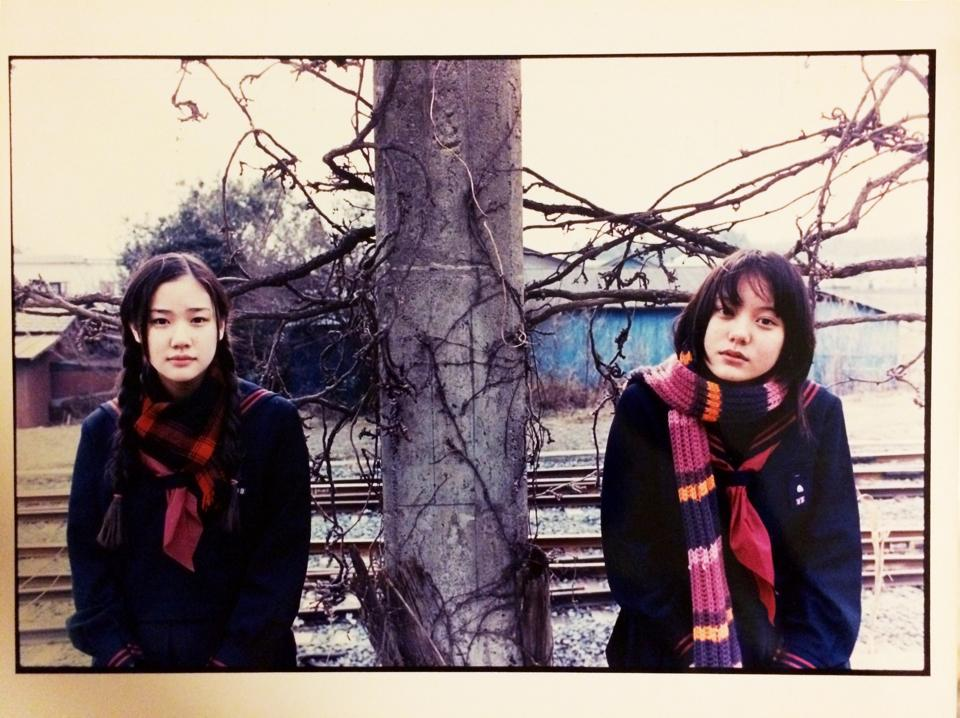
\includegraphics[width=\linewidth]{graph.jpg}
  \caption{How beautiful they are}\label{twoprettygirls}
\endminipage\hfill
\minipage{0.5\textwidth}
  
\includegraphics[width=\linewidth]{graph1.jpg}
  \caption{How pretty she is}\label{koreangirl}
\endminipage\hfill
\end{figure}

\newpage
Python Code:
\begin{lstlisting}
#!/usr/bin/env python3

import math
import numpy as np
import matplotlib.pyplot as plt
from scipy.signal import lti, step2

# 1st question
num = [1]
den = [1, 0.5, 2]

if i is a:
  print('hello')
else:
  print('world')
transfer = lti(num, den)
t, y = step2(transfer)

fig = plt.figure()
plt.subplot(111)
plt.plot(t, y)
plt.xlabel('Time')
plt.ylabel('Output')
plt.show()
\end{lstlisting}

And this is how you inline C code, \inlinecode{C}{(counter<<7) & 0x80)}.

\newpage
\section{Task 2}
a) $R_1=0.1k, R_2=2.2k, C_1=0.1\mu$

Just a random text here.

b) $R_1=1k, R_2=100k, C_1=1\mu$

\begin{figure}[!htb]
\minipage{0.5\textwidth}
  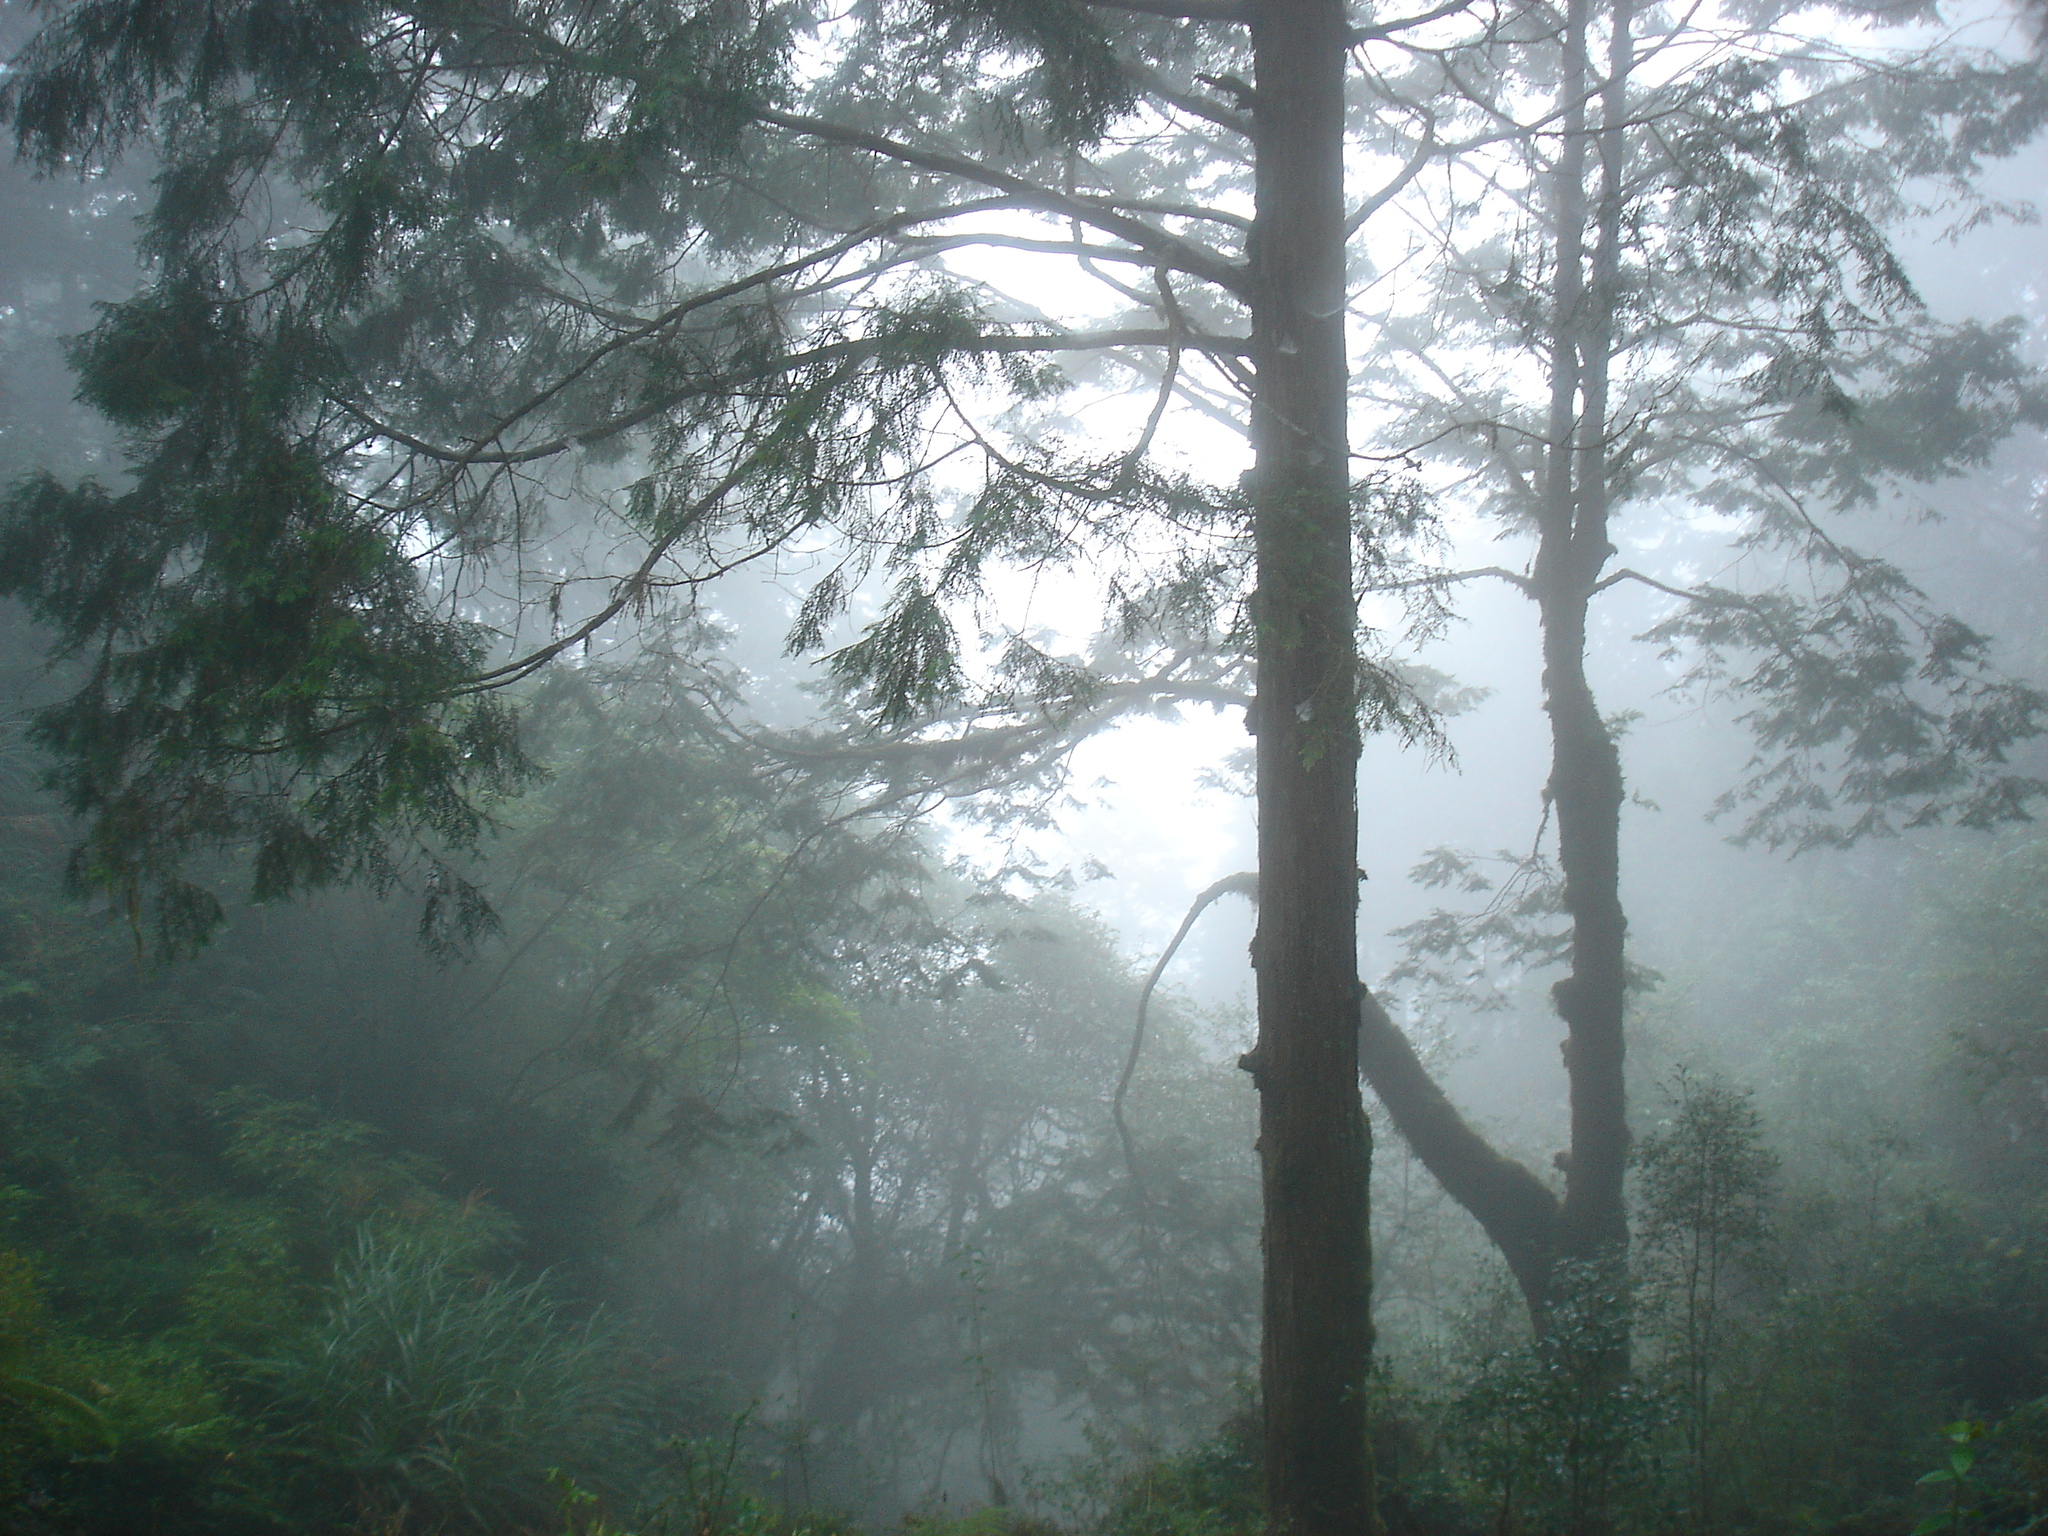
\includegraphics[width=\linewidth]{graph2.jpg}
  \caption{An unknown forest in Taiwan}\label{forest_taiwan}
\endminipage\hfill
\end{figure}

A geostationary orbit, often referred to as a geosynchronous equatorial orbit[1] (GEO), is a circular geosynchronous orbit 35,786 km (22,236 mi) above Earth's equator and following the direction of Earth's rotation.

\begin{figure}[!htb]
\minipage{0.5\textwidth}
  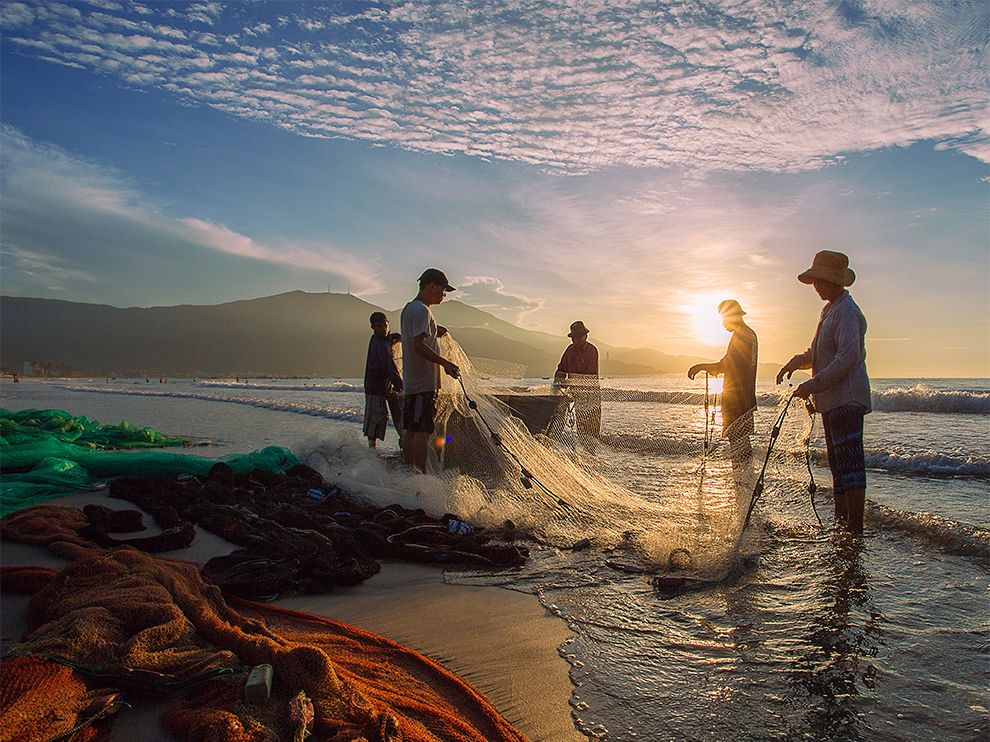
\includegraphics[width=\linewidth]{graph3.jpg}
  \caption{Fishman in the morning}\label{fishman_taiwan}
\endminipage\hfill
\end{figure}

\newpage
In celestial mechanics, the mean anomaly is an angle used in calculating the position of a body in an elliptical orbit in the classical two-body problem. It is the angular distance from the pericenter which a fictitious body would have if it moved in a circular orbit, with constant speed, in the same orbital period as the actual body in its elliptical orbit.
\begin{figure}[!htb]
\minipage{0.5\textwidth}
  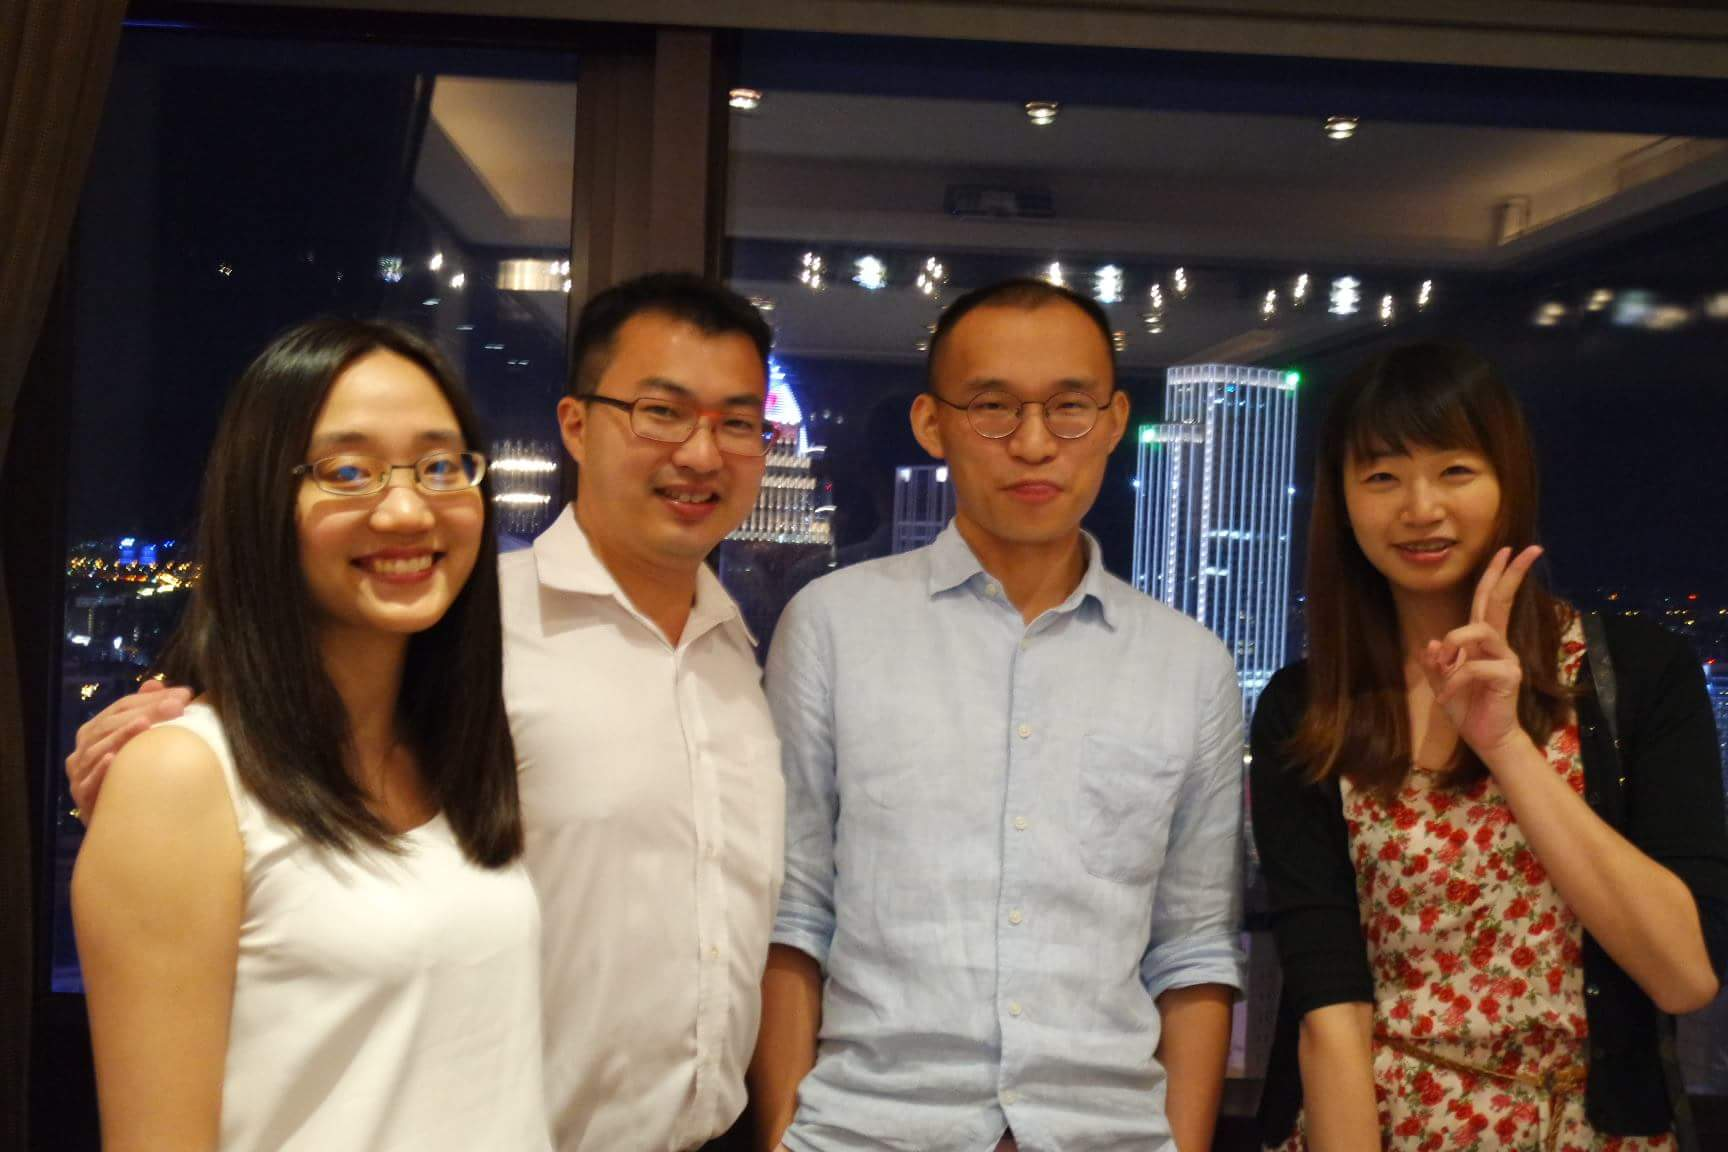
\includegraphics[width=\linewidth]{graph4.jpg}
  \caption{Photo with friends from Taiwan and China}\label{wedding_friends}
\endminipage\hfill
\end{figure}

\begin{figure}[!htb]
\minipage{0.5\textwidth}
  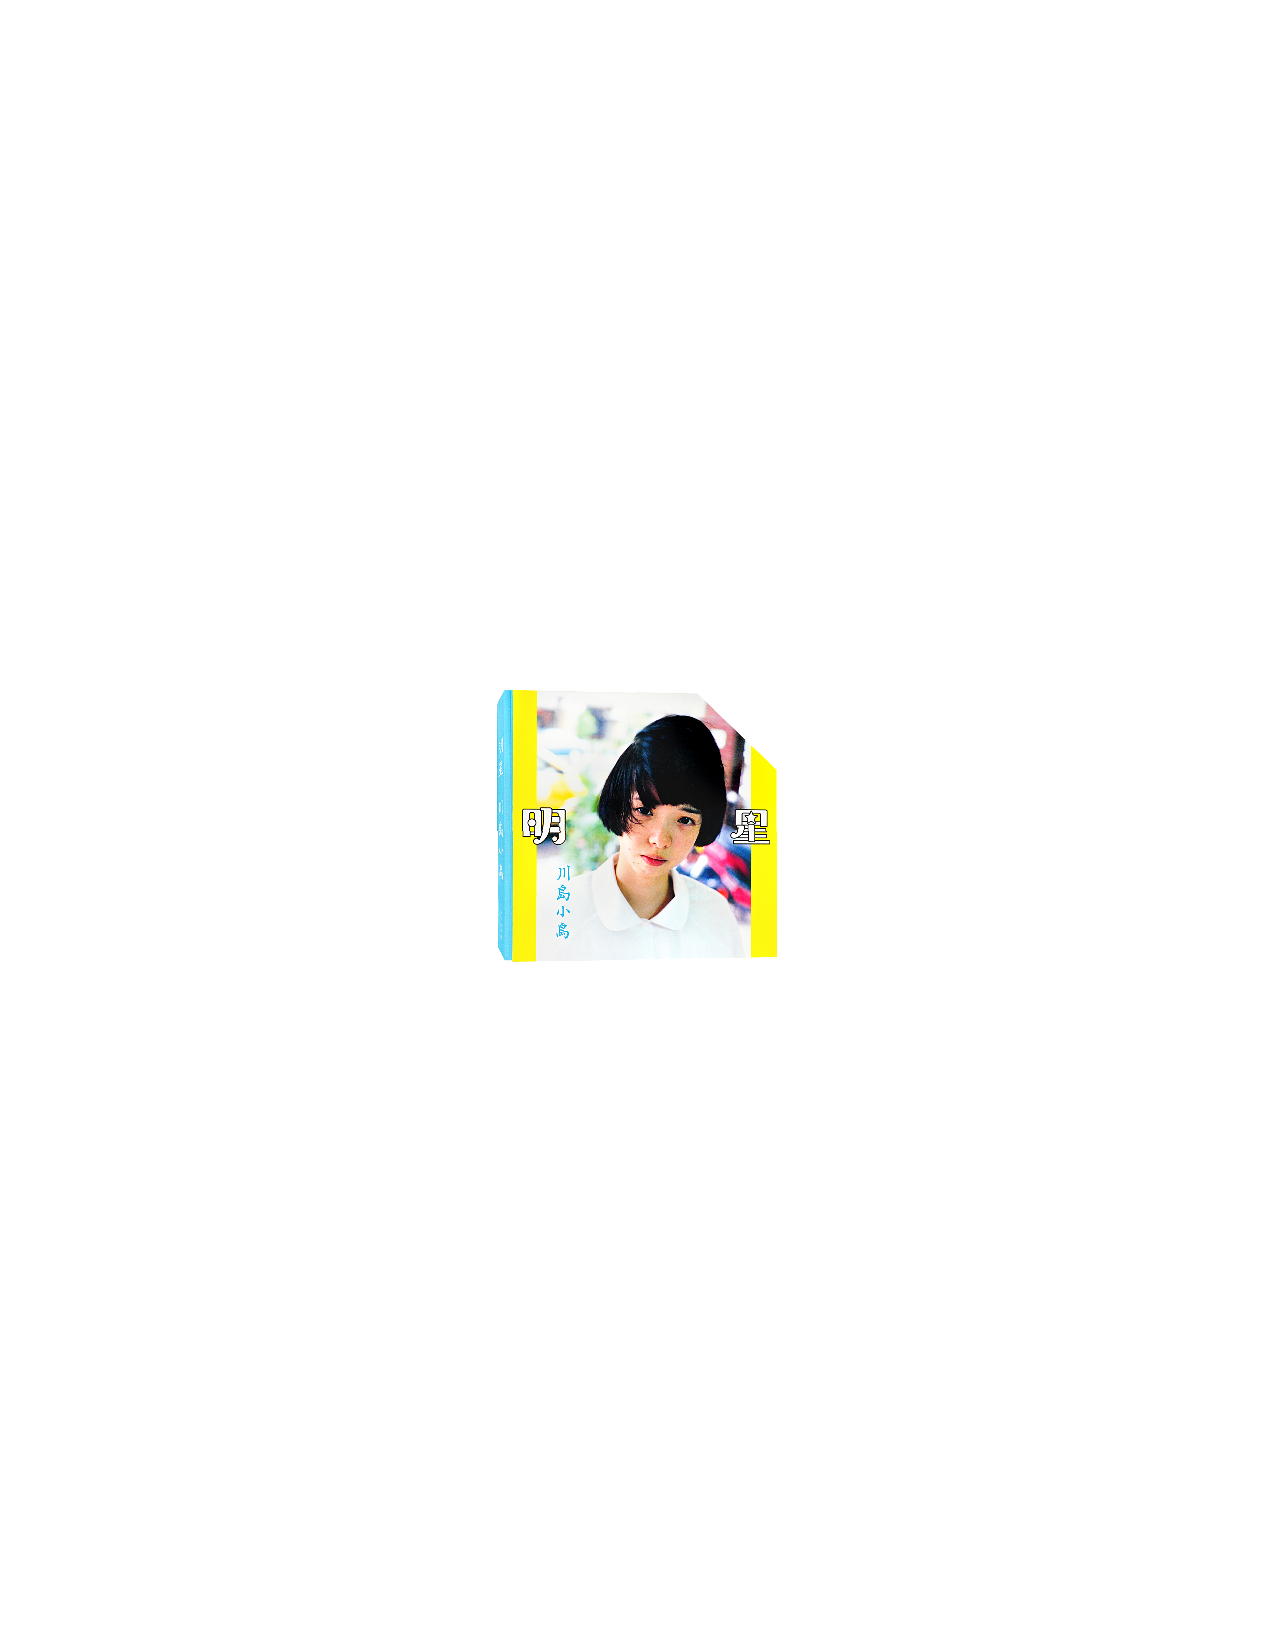
\includegraphics[width=\linewidth]{graph5.pdf}
  \caption{An astounding image of a girl}\label{taiwan_girl}
\endminipage\hfill
\end{figure}

% --------------------------------------------------------------
%     You don't have to mess with anything below this line.
% --------------------------------------------------------------

\end{document}